  \clearpage
  %%%%%%%%%%%%%%%%%%%%%%%%%%%%%%%%%%%%%%%%%%%%%%%%%%%%%%%%%%%%%%%%%%%%%%%%%%%%%%%%%
  %%        %%%        %%%        %%%        %%%        %%%         %%%  %%%%  %%%
  %%  %%%%%%%%%  %%%%%%%%%  %%%%%%%%%%%%  %%%%%%%%%  %%%%%%  %%%%%  %%%    %%  %%%
  %%        %%%        %%%  %%%%%%%%%%%%  %%%%%%%%%  %%%%%%  %%%%%  %%%  %  %  %%%
  %%%%%%%%  %%%  %%%%%%%%%  %%%%%%%%%%%%  %%%%%%%%%  %%%%%%  %%%%%  %%%  %%    %%%
  %%        %%%        %%%        %%%%%%  %%%%%%        %%%         %%%  %%%   %%%
  %%%%%%%%%%%%%%%%%%%%%%%%%%%%%%%%%%%%%%%%%%%%%%%%%%%%%%%%%%%%%%%%%%%%%%%%%%%%%%%%%
 \section{\texttt{TRandom}と\texttt{TCanvas}}

 乱数とキャンバスの操作に出会う。

 \begin{itembox}{\texttt{canran.cpp}}
\begin{verbatim}
	#include "TCanvas.h"
	#include "TH1.h"
	#include "TRandom3.h"
	#include "TStyle.h"
	TCanvas *canran(){
	TCanvas *c1 = new TCanvas("c1","c1",600,600) ;
	TRandom3 *r = new TRandom3();
	TH1D *h = new TH1D("h","h-title;x;y",100,-5,5) ;
	for(int i = 0 ; i<100000 ; i++){
	h->Fill(r->Uniform(-3.,3.)) ;
	}
	h->Draw("HE") ;
	c1->SaveAs("c1.eps") ;
	return c1 ;
	}
\end{verbatim}
 \end{itembox}


 \begin{figure}[htbp]
  \begin{center}
   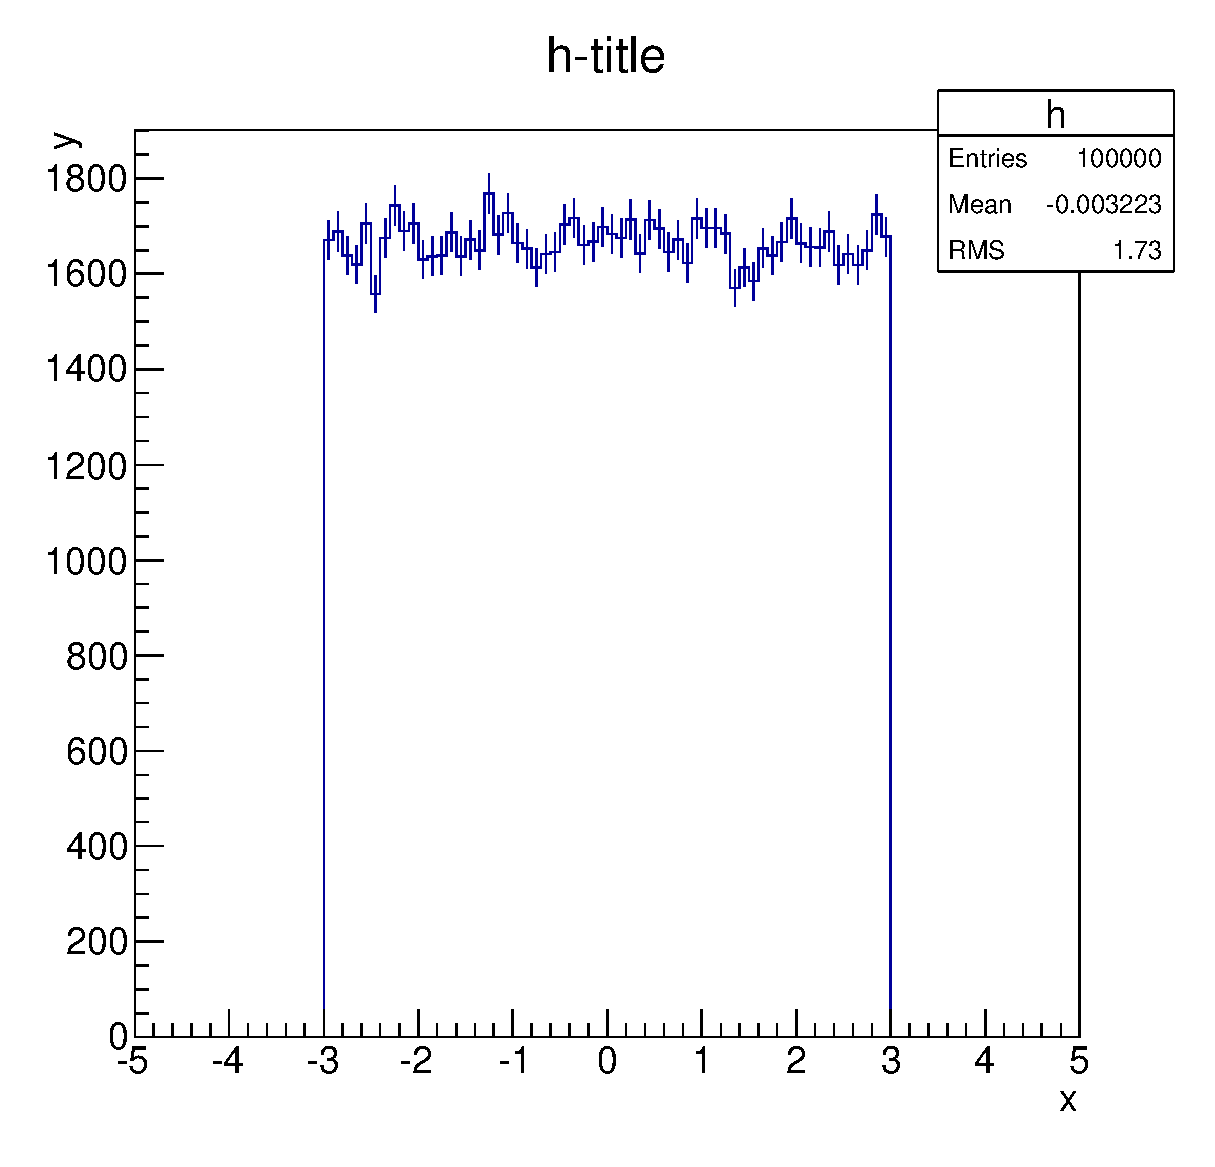
\includegraphics[width = 90mm] {./picture/canrancanvas1.eps}
  \end{center}
  \caption{\texttt{canran.cpp}の実行結果}
  \label{Fig:canrancanvas1}
 \end{figure}


  \subsection{練習}

  \begin{enumerate}

   \item プログラムの各行を説明せよ。
	 \begin{description}
	  \item[ヒント] メルセンヌツイスタとはメルセンヌ数という数の特徴を用いた乱数生成子のこと。
	  \item[ヒント] \url{http://root.cern.ch/root/htmldoc/TRandom.html}
	  \item[ヒント] \url{http://root.cern.ch/root/htmldoc/TRandom3.html}
	 \end{description}

   \item 今は
	 \verb|h->Fill(r->Uniform(-1.,1.)) ;|としているが、
	 \verb|h->Fill(r->Exp(1.)) ;|、
	 \verb|h->Fill(r->Gaus(1.,1.)) ;|、
	 \verb|h->Fill(r->Binomial(3,0.3)) ;|、
	 \verb|h->Fill(r->PoissonD(1)) ;|
	 などとした時の挙動を確かめよ。
	 \begin{description}
	  \item[ヒント] これを気に幾つかの基本的な確率分布について調べよ。
	  \item[ヒント] \url{http://root.cern.ch/root/htmldoc/TRandom.html#TRandom:Exp}
	  \item[ヒント] \url{http://root.cern.ch/root/htmldoc/TRandom.html#TRandom:Gaus}
	  \item[ヒント] \url{http://root.cern.ch/root/htmldoc/TRandom.html#TRandom:Binomial}
	  \item[ヒント] \url{http://root.cern.ch/root/htmldoc/TRandom.html#TRandom:Poisson}
	 \end{description}

   \item hist1を繰り返し実行した時にヒストグラムに変化があるかどうか検証せよ。
	 変化がない場合、この原因を突き止めて実行毎に違うヒストグラムが出来上がるような仕様へ変更せよ。
	 \begin{description} 
	  \item[ヒント] \url{http://root.cern.ch/root/htmldoc/TRandom.html#TRandom:TRandom}
	  \item[ヒント] \url{http://root.cern.ch/root/htmldoc/TRandom.html#TRandom:SetSeed}
	 \end{description}
  \end{enumerate}

  \subsection{解答例}

  \begin{enumerate}

   \item プログラムの各行を説明せよ。

   \item 今は
	 \verb|h->Fill(r->Uniform(-1.,1.)) ;|としているが、
	 \verb|h->Fill(r->Exp(1.)) ;|、
	 \verb|h->Fill(r->Gaus(1.,1.)) ;|、
	 \verb|h->Fill(r->Binomial(3,0.3)) ;|、
	 \verb|h->Fill(r->PoissonD(1)) ;|
	 などとした時の挙動を確かめよ。

   \item hist1を繰り返し実行した時にヒストグラムに変化があるかどうか検証せよ。
	 変化がない場合、この原因を突き止めて実行毎に違うヒストグラムが出来上がるような仕様へ変更せよ。
	 \begin{itembox}{\texttt{canransol1.cpp}}
\begin{verbatim}
	...
	TCanvas *canransol1(){
	TCanvas *c1 = new TCanvas("c1","c1",600,600) ;
	TRandom3 *r = new TRandom3() ;
	r->SetSeed(unsigned (time(NULL))) ;
	...
	}
\end{verbatim}
	 \end{itembox}

  \end{enumerate}
